\documentclass[11pt,oneside]{article}
\usepackage[T1]{fontenc}
\usepackage[utf8]{inputenc}
% \usepackage{lmodern}
%\usepackage[adobe-utopia,uppercase=upright,greeklowercase=upright]{mathdesign}
\usepackage[adobe-utopia]{mathdesign}
%\usepackage{minionpro}
% \usepackage{pifont}
% \usepackage{amssymb}
\usepackage{amsmath}
\usepackage[francais]{babel}
% \usepackage[francais]{varioref}
\usepackage[dvips]{graphicx}

\usepackage{framed}
\usepackage[normalem]{ulem}
\usepackage{fancyhdr}
\usepackage{titlesec}
\usepackage{vmargin}
\usepackage{longtable}

\usepackage{ifthen}


%\usepackage{epsfig}
\usepackage{subfig}

\usepackage{multirow}
\usepackage{multicol} % Portions de texte en colonnes
\usepackage{flafter}%floatants après la référence



\usepackage{color}
\usepackage{colortbl}


\definecolor{gris25}{gray}{0.75}
\definecolor{bleu}{RGB}{18,33,98}
\definecolor{bleuf}{RGB}{42,94,171}
\definecolor{bleuc}{RGB}{231,239,247}
\definecolor{rougef}{RGB}{185,18,27}
\definecolor{rougec}{RGB}{255,230,231}
\definecolor{vertf}{RGB}{103,126,82}
\definecolor{vertc}{RGB}{220,255,191}
\definecolor{violetf}{RGB}{112,48,160}
\definecolor{violetc}{RGB}{230,224,236}

\newenvironment{sci}[1][\hsize]%
{%
    \def\FrameCommand%
    {%
%\rotatebox{90}{\textit{\textsf{Scilab}}\includegraphics[height=.8cm]{png/logo_scilab}} 
\rotatebox{90}{\includegraphics[height=.6cm]{png/logo_scilab}} 
        {\color{violetf}\vrule width 3pt}%
        \hspace{0pt}%must no space.
        \fboxsep=\FrameSep\colorbox{violetc}%
    }%
    \MakeFramed{\hsize #1 \advance\hsize-\width\FrameRestore}%
}%
{\endMakeFramed}%

\newenvironment{pseudo}[1][\hsize]%
{%
    \def\FrameCommand%
    {%
\rotatebox{90}{\textit{\textsf{Pseudo Code}}} 
        {\color{violetf}\vrule width 3pt}%
        \hspace{0pt}%must no space.
        \fboxsep=\FrameSep\colorbox{violetc}%
    }%
    \MakeFramed{\hsize #1 \advance\hsize-\width\FrameRestore}%
}%
{\endMakeFramed}%

\newenvironment{py}[1][\hsize]%
{%
    \def\FrameCommand%
    {%
%\rotatebox{90}{\textit{\textsf{Python}}} 
\rotatebox{90}{\includegraphics[height=.6cm]{png/logo_python}} 
        {\color{violetf}\vrule width 3pt}%
        \hspace{0pt}%must no space.
        \fboxsep=\FrameSep\colorbox{violetc}%
    }%
    \MakeFramed{\hsize #1 \advance\hsize-\width\FrameRestore}%
}%
{\endMakeFramed}%


\newenvironment{corrige}[1][\hsize]%
{%
    \def\FrameCommand
    {%
\rotatebox{90}{\textit{\textsf{Correction}}} 
        {\color{violetf}\vrule width 3pt}%
        \hspace{0pt}%must no space.
        \fboxsep=\FrameSep\colorbox{violetc}%
    }%
    \MakeFramed{\hsize#1\advance\hsize-\width\FrameRestore}%
}%
{\endMakeFramed}%



\newenvironment{rem}[1][\hsize]%
{%
    \def\FrameCommand
    {%
\rotatebox{90}{\textit{\textsf{Remarque}}} 
        {\color{bleuf}\vrule width 3pt}%
        \hspace{0pt}%must no space.
        \fboxsep=\FrameSep\colorbox{bleuc}%
    }%
    \MakeFramed{\hsize#1\advance\hsize-\width\FrameRestore}%
}%
{\endMakeFramed}%


\newenvironment{savoir}[1][\hsize]%
{%
    \def\FrameCommand
    {%
\rotatebox{90}{\textit{\textsf{Savoir}}} 
        {\color{bleuf}\vrule width 3pt}%
        \hspace{0pt}%must no space.
        \fboxsep=\FrameSep\colorbox{bleuc}%
    }%
    \MakeFramed{\hsize#1\advance\hsize-\width\FrameRestore}%
}%
{\endMakeFramed}%

\newenvironment{prob}[1][\hsize]%
{%
    \def\FrameCommand%
    {%
\rotatebox{90}{\textit{\textsf{ Problématique}}} 
        {\color{rougef}\vrule width 3pt}%
        \hspace{0pt}%must no space.
        \fboxsep=\FrameSep\colorbox{rougec}%
    }%
    \MakeFramed{\hsize#1\advance\hsize-\width\FrameRestore}%
}%
{\endMakeFramed}%

\newenvironment{obj}[1][\hsize]%
{%
    \def\FrameCommand%
    {%
\rotatebox{90}{\textit{\textsf{ $\;$}}} 
        {\color{rougef}\vrule width 3pt}%
        \hspace{0pt}%must no space.
        \fboxsep=\FrameSep\colorbox{rougec}%
    }%
    \MakeFramed{\hsize#1\advance\hsize-\width\FrameRestore}%
}%
{\endMakeFramed}%

\newenvironment{defi}[1][\hsize]%
{%
    \def\FrameCommand%
    {%
\rotatebox{90}{\textit{\textsf{Définition\\}}} 
        {\color{bleuf}\vrule width 3pt}%
        \hspace{0pt}%must no space.
        \fboxsep=\FrameSep\colorbox{bleuc}%
    }%
    \MakeFramed{\hsize#1\advance\hsize-\width\FrameRestore}%
}%
{\endMakeFramed}%


\newenvironment{demo}[1][\hsize]%
{%
    \def\FrameCommand%
    {%
\rotatebox{90}{\textit{\textsf{Démonstration\\}}} 
        {\color{bleuf}\vrule width 3pt}%
        \hspace{0pt}%must no space.
        \fboxsep=\FrameSep\colorbox{bleuc}%
    }%
    \MakeFramed{\hsize#1\advance\hsize-\width\FrameRestore}%
}%
{\endMakeFramed}%


\newenvironment{hypo}[1][\hsize]%
{%
    \def\FrameCommand%
    {%
\rotatebox{90}{\textit{\textsf{Hypothèse\\}}} 
        {\color{bleuf}\vrule width 3pt}%
        \hspace{0pt}%must no space.
        \fboxsep=\FrameSep\colorbox{bleuc}%
    }%
    \MakeFramed{\hsize#1\advance\hsize-\width\FrameRestore}%
}%
{\endMakeFramed}%


\newenvironment{prop}[1][\hsize]%
{%
    \def\FrameCommand%
    {%
\rotatebox{90}{\textit{\textsf{Propriété\\}}} 
        {\color{bleuf}\vrule width 3pt}%
        \hspace{0pt}%must no space.
        \fboxsep=\FrameSep\colorbox{bleuc}%
    }%
    \MakeFramed{\hsize#1\advance\hsize-\width\FrameRestore}%
}%
{\endMakeFramed}%

\newenvironment{props}[1][\hsize]%
{%
    \def\FrameCommand%
    {%
\rotatebox{90}{\textit{\textsf{Propriétés\\}}} 
        {\color{bleuf}\vrule width 3pt}%
        \hspace{0pt}%must no space.
        \fboxsep=\FrameSep\colorbox{bleuc}%
    }%
    \MakeFramed{\hsize#1\advance\hsize-\width\FrameRestore}%
}%
{\endMakeFramed}%

\newenvironment{exemple}[1][\hsize]%
{%
    \def\FrameCommand%
    {%
\rotatebox{90}{\textit{\textsf{Exemple\\}}} 
        {\color{vertf}\vrule width 3pt}%
        \hspace{0pt}%must no space.
        \fboxsep=\FrameSep\colorbox{vertc}%
    }%
    \MakeFramed{\hsize#1\advance\hsize-\width\FrameRestore}%
}%
{\endMakeFramed}%

\newenvironment{resultat}[1][\hsize]%
{%
    \def\FrameCommand%
    {%
\rotatebox{90}{\textit{\textsf{Résultat\\}}} 
        {\color{rougef}\vrule width 3pt}%
        \hspace{0pt}%must no space.
        \fboxsep=\FrameSep\colorbox{rougec}%
    }%
    \MakeFramed{\hsize#1\advance\hsize-\width\FrameRestore}%
}%
{\endMakeFramed}%

\newenvironment{methode}[1][\hsize]%
{%
    \def\FrameCommand%
    {%
\rotatebox{90}{\textit{\textsf{Méthode\\}}} 
        {\color{rougef}\vrule width 3pt}%
        \hspace{0pt}%must no space.
        \fboxsep=\FrameSep\colorbox{rougec}%
    }%
    \MakeFramed{\hsize#1\advance\hsize-\width\FrameRestore}%
}%
{\endMakeFramed}%

\newenvironment{theo}[1][\hsize]%
{%
    \def\FrameCommand%
    {%
\rotatebox{90}{\textit{\textsf{Théorème\\}}} 
        {\color{rougef}\vrule width 3pt}%
        \hspace{0pt}%must no space.
        \fboxsep=\FrameSep\colorbox{rougec}%
    }%
    \MakeFramed{\hsize#1\advance\hsize-\width\FrameRestore}%
}%
{\endMakeFramed}%

\newenvironment{warn}[1][\hsize]%
{%
    \def\FrameCommand%
    {%
\rotatebox{90}{\textit{\textsf{Attention\\}}} 
        {\color{rougef}\vrule width 3pt}%
        \hspace{0pt}%must no space.
        \fboxsep=\FrameSep\colorbox{rougec}%
    }%
    \MakeFramed{\hsize#1\advance\hsize-\width\FrameRestore}%
}%
{\endMakeFramed}%

% \usepackage{pstricks}
%\usepackage{minitoc}
% \setcounter{minitocdepth}{4}

\setcounter{tocdepth}{2}

% \mtcselectlanguage{french} 

%\usepackage{draftcopy}% "Brouillon"
% \usepackage{floatflt}
\usepackage{psfrag}
%\usepackage{listings} % Permet d'insérer du code de programmation
\renewcommand{\baselinestretch}{1.2}

% Changer la numérotation des figures :
% ------------------------------------
% \makeatletter
% \renewcommand{\thefigure}{\ifnum \c@section>\z@ \thesection.\fi
%  \@arabic\c@figure}
% \@addtoreset{figure}{section}
% \makeatother
 


%%%%%%%%%%%%
% Définition des vecteurs %
%%%%%%%%%%%%
 \newcommand{\vect}[1]{\overrightarrow{#1}}

%%%%%%%%%%%%
% Définition des torseusr %
%%%%%%%%%%%%

 \newcommand{\torseur}[1]{%
\left\{{#1}\right\}
}

\newcommand{\torseurcin}[3]{%
\left\{\mathcal{#1} \left(#2/#3 \right) \right\}
}

\newcommand{\torseurstat}[3]{%
\left\{\mathcal{#1} \left(#2\rightarrow #3 \right) \right\}
}

 \newcommand{\torseurc}[8]{%
%\left\{#1 \right\}=
\left\{
{#1}
\right\}
 = 
\left\{%
\begin{array}{cc}%
{#2} & {#5}\\%
{#3} & {#6}\\%
{#4} & {#7}\\%
\end{array}%
\right\}_{#8}%
}

 \newcommand{\torseurcol}[7]{
\left\{%
\begin{array}{cc}%
{#1} & {#4}\\%
{#2} & {#5}\\%
{#3} & {#6}\\%
\end{array}%
\right\}_{#7}%
}

 \newcommand{\torseurl}[3]{%
%\left\{\mathcal{#1}\right\}_{#2}=%
\left\{%
\begin{array}{l}%
{#1} \\%
{#2} %
\end{array}%
\right\}_{#3}%
}

 \newcommand{\vectv}[3]{%
\vect{V\left( {#1} \in {#2}/{#3}\right)}
}


\newcommand{\vectf}[2]{%
\vect{R\left( {#1} \rightarrow {#2}\right)}
}

\newcommand{\vectm}[3]{%
\vect{\mathcal{M}\left( {#1}, {#2} \rightarrow {#3}\right)}
}


 \newcommand{\vectg}[3]{%
\vect{\Gamma \left( {#1} \in {#2}/{#3}\right)}
}

 \newcommand{\vecto}[2]{%
\vect{\Omega\left( {#1}/{#2}\right)}
}
% }$$\left\{\mathcal{#1} \right\}_{#2} =%
% \left\{%
% \begin{array}{c}%
%  #3 \\%
%  #4 %
% \end{array}%
% \right\}_{#5}}

%  ------------------------------------------
% | Modification du formatage des sections : | 
%  ------------------------------------------

% Grands titres :
% ---------------

\newcommand{\titre}[1]{%
\begin{center}
      \bigskip
      \rule{\textwidth}{1pt}
      \par\vspace{0.1cm}
      
      \textbf{\large #1}
      \par\rule{\textwidth}{1pt}
    \end{center}
    \bigskip
  }

% Supprime le numéro du chapitre dans la numérotation des sections:
% -----------------------------------------------------------------
\makeatletter
\renewcommand{\thesection}{\@arabic\c@section}
\makeatother


% \titleformat{\chapter}[display]
% {\normalfont\Large\filcenter}
% {}
% {1pc}
% {\titlerule[1pt]
%   \vspace{1pc}%
%   \Huge}[\vspace{1ex}%
% \titlerule]


%%%% Chapitres Comme PY Pechard %%%%%%%%%
% numéro du chapitre
\DeclareFixedFont{\chapnumfont}{OT1}{phv}{b}{n}{80pt}
% pour le mot « Chapitre »
\DeclareFixedFont{\chapchapfont}{OT1}{phv}{m}{it}{40pt}
% pour le titre
\DeclareFixedFont{\chaptitfont}{T1}{phv}{b}{n}{25pt}

\definecolor{gris}{gray}{0.75}
\titleformat{\chapter}[display]%
	{\sffamily}%
	{\filleft\chapchapfont\color{gris}\chaptertitlename\
	\\
	\vspace{12pt}
	\chapnumfont\thechapter}%
	{16pt}%
	{\filleft\chaptitfont}%
	[\vspace{6pt}\titlerule\titlerule\titlerule]

%%%%  Fin Chapitres Comme PY Pechard %%%%%%%%%


% Section, subsection, subsubsection sans serifs :
% % ----------------------------------------------

% \makeatletter
% \renewcommand{\section}{\@startsection{section}{0}{0mm}%
% {\baselineskip}{.3\baselineskip}%
% {\normalfont\sffamily\Large\textbf}}%
% \makeatother

\makeatletter
\renewcommand{\@seccntformat}[1]{{\textcolor{bleu}{\csname
the#1\endcsname}\hspace{0.5em}}}
\makeatother

\makeatletter
\renewcommand{\section}{\@startsection{section}{1}{\z@}%
                       {-4ex \@plus -1ex \@minus -.4ex}%
                       {1ex \@plus.2ex }%
                       {\normalfont\Large\sffamily\bfseries}}%
\makeatother
 
\makeatletter
\renewcommand{\subsection}{\@startsection {subsection}{2}{\z@}
                          {-3ex \@plus -0.1ex \@minus -.4ex}%
                          {0.5ex \@plus.2ex }%
                          {\normalfont\large\sffamily\bfseries}}
\makeatother
 
\makeatletter
\renewcommand{\subsubsection}{\@startsection {subsubsection}{3}{\z@}
                          {-2ex \@plus -0.1ex \@minus -.2ex}%
                          {0.2ex \@plus.2ex }%
                          {\normalfont\large\sffamily\bfseries}}
\makeatother
 
\makeatletter             
\renewcommand{\paragraph}{\@startsection{paragraph}{4}{\z@}%
                                    {-2ex \@plus-.2ex \@minus .2ex}%
                                    {0.1ex}%               
{\normalfont\sffamily\bfseries}}
\makeatother
 

\makeatletter             
\renewcommand{\subparagraph}{\@startsection{subparagraph}{5}{\z@}%
                                    {-2ex \@plus-.2ex \@minus .2ex}%
                                    {0.1ex}%               
{\normalfont\bfseries Question }}
\makeatother

\renewcommand{\thesubparagraph}{\arabic{subparagraph}} 
%
\makeatletter
%\renewcommand{\subparagraph}{\@startsection{subparagraph}{5}{\z@}%
%                                       {-2ex \@plus-.1ex \@minus .2ex}%
%                                       {0.1ex}%
%				    {\normalfont\normalsize\sffamily\bfseries}}
%\makeatletter
% \makeatletter
% \renewcommand{\subsection}{\@startsection{subsection}{1}{2mm}%
% {\baselineskip}{.3\baselineskip}%
% {\normalfont\sffamily\large\textbf}}%
% \makeatother
% 
% \makeatletter
% \renewcommand{\subsubsection}{\@startsection{subsubsection}{2}{4mm}%
% {\baselineskip}{.15\baselineskip}%
% {\normalfont\sffamily\large\textbf}}%
% \makeatother
% 
% \makeatletter
% \renewcommand{\paragraph}{\@startsection{paragraph}{3}{6mm}%
% {\baselineskip}{.15\baselineskip}%
% {\normalfont\sffamily\large\textbf}}%
% \makeatother
 
\setcounter{secnumdepth}{5}


%  --------
% | Marges |
%  --------


% \setmarginsrb{2.5cm}{1.5cm}{2.5cm}{2cm}{1cm}{1cm}{1cm}{1cm}
\setmarginsrb{1.5cm}{1cm}{1cm}{1.5cm}{1cm}{1cm}{1cm}{1cm}

% Changer les marges localement :
% -----------------------------
\newenvironment{changemargin}[2]{\begin{list}{}{%
\setlength{\topsep}{0pt}%
\setlength{\leftmargin}{0pt}%
\setlength{\rightmargin}{0pt}%
\setlength{\listparindent}{\parindent}%
\setlength{\itemindent}{\parindent}%
\setlength{\parsep}{0pt plus 1pt}%
\addtolength{\leftmargin}{#1}%
\addtolength{\rightmargin}{#2}%
}\item }{\end{list}}



\usepackage{pst-solides3d}
\usepackage{titletoc}
\titlecontents{chapter}[+3pc]
  {\addvspace{10pt}\sffamily\bfseries}
{\contentslabel[{\pscirclebox[fillstyle=solid,fillcolor=gray!25,
linecolor=gray!25,framesep=4pt]{\textcolor{white}{\thecontentslabel}}}]{2.5pc}}
  {}
  {\dotfill \normalfont\thecontentspage\ }

\titlecontents{section}[3pc]
  {\addvspace{2pt}\sffamily}
  {\contentslabel[\thecontentslabel]{1.8pc}}
  {}
  {\dotfill \normalfont\thecontentspage\ }

\titlecontents{subsection}[5pc]
  {\addvspace{2pt}\sffamily}
  {\contentslabel[\thecontentslabel]{1.8pc}}
  {}
  {\dotfill \normalfont\thecontentspage\ }

\titlecontents{subsubsection}[8pc]
  {\addvspace{2pt}\sffamily}
  {\contentslabel[\thecontentslabel]{3pc}}
  {}
  {\dotfill \normalfont\thecontentspage\ }
%{\;\titlerule\;\normalfont\thecontentspage\ }

\titlecontents{paragraph}[9pc]
  {\addvspace{2pt}\sffamily}
  {\contentslabel[\thecontentslabel]{3.5pc}}
  {}
  {\dotfill \normalfont\thecontentspage\ }




\usepackage[%
    pdftitle={SLCI -- Modélisation par transformée de Laplace -- Applications},
    pdfauthor={Xavier Pessoles},
    colorlinks=true,
    linkcolor=blue,
    citecolor=magenta]{hyperref}



% \makeatletter \let\ps@plain\ps@empty \makeatother
%% DEBUT DU DOCUMENT
%% =================
\sloppy
\hyphenpenalty 10000

\newcommand{\Pointilles}[1][3]{%
\multido{}{#1}{\makebox[\linewidth]{\dotfill}\\[\parskip]
}}


\begin{document}


\newboolean{prof}
\setboolean{prof}{true}
%------------- En tetes et Pieds de Pages ------------
\pagestyle{fancy}
\renewcommand{\headrulewidth}{0pt}

\fancyhead{}
\fancyhead[L]{%
\noindent\noindent\begin{minipage}[c]{2.6cm}
%Lycée Rouvière PTSI

\includegraphics[width=2cm]{png/logo_ptsi.png}%
\end{minipage}
}

\fancyhead[C]{\rule{12cm}{.5pt}}

\fancyhead[R]{%
\begin{minipage}[c]{3cm}
\begin{flushright}
\footnotesize{\textit{\textsf{Sciences Industrielles\\ de l'Ingénieur}}}%
\end{flushright}
\end{minipage}
}

\renewcommand{\footrulewidth}{0.2pt}

\fancyfoot[C]{\footnotesize{\bfseries \thepage}}
\fancyfoot[L]{\footnotesize{2013 -- 2014} \\ X. \textsc{Pessoles}}
\ifthenelse{\boolean{prof}}{%
\fancyfoot[R]{\footnotesize{CI 2 : SLCI -- Applications} \\ \footnotesize{Ch. 2 : Modélisation -- P}}
}{%
\fancyfoot[R]{\footnotesize{CI 2 : SLCI -- Applications} \\ \footnotesize{Ch. 2 : Modélisation -- E}}
}


%\begin{center}
%\textit{Centre d'intérêt}
%\end{center}



\begin{center}
 \Large\textsc{CI 2 -- SLCI : Étude du comportement des Systèmes Linéaires Continus Invariants}
\end{center}

\begin{center}
 \large\textsc{Chapitre 2 -- Modélisation des Systèmes Linéaires Continus Invariants}

 \large\textsc{Transformée de Laplace} 
\end{center}

\begin{center}
\textsc{Exercices d'application} 

\end{center}

\begin{flushright}
\textit{D'après ressources de Jean-Pierre Pupier et Florestan Mathurin.} 
\end{flushright}
\vspace{.5cm}

\subsection*{Exercice 1}
\setcounter{subparagraph}{0}
On souhaite résoudre l'équation différentielle suivante : 
$$
\dfrac{de(t)}{dt}+e(t) = \dfrac{d^3s(t)}{dt^3}+\dfrac{d^2s(t)}{dt^2}+\dfrac{ds(t)}{dt}
$$
$e(t)$ est l'entrée du système, $s(t)$ la sortie.

On se place dans les conditions de Heaviside, c'est-à-dire qu'on considère que $s(t)$, $e(t)$ et leurs dérivées successives sont nulles en $t=0$. 

\subparagraph{}
\textit{En utilisant les résultats sur la transformée de Laplace, donner l'équation différentielle dans le domaine de Laplace.}

\ifthenelse{\boolean{prof}}{
\begin{corrige}
En utilisant la propriété de la transformée de Laplace de la dérivée, 
$\mathcal{L}\left[ \dfrac{df(t)}{dt}\right]=pF(p)-f(0^+)$. Étant dans les conditions de Heaviside, on a donc :
$$
pE(p)+E(p)=p^3S(p)+p^2S(p)+pS(p)
$$


\end{corrige}
}{}

Pour la suite on considère que le système est soumis à une entrée $e(t)$ indicielle. 

\subparagraph{}
\textit{Donner l'allure graphique d'une entrée indicielle. Donner sa forme dans le domaine temporel puis dans le domaine de Laplace. En déduire $S(p)$.}
\ifthenelse{\boolean{prof}}{
\begin{corrige}
Pour $t\in\mathbb{R}^+_*$, on a $e(t)=1$, sinon $e(t)=0$.

Dans le domaine de Laplace, $E(p)=\dfrac{1}{p}$.

En conséquence, 
$$
S(p)=\dfrac{1+p}{p^3+p^2+p}
$$
\end{corrige}
}{}



\subparagraph{}
\textit{Déterminer les valeurs finales et initiales de $s(t)$.}
\ifthenelse{\boolean{prof}}{
\begin{corrige}
D'après le théorème de la valeur initiale, 
$$
\lim\limits_{t\rightarrow 0} s(t) 
= \lim\limits_{p\rightarrow +\infty} pS(p)
= \lim\limits_{p\rightarrow +\infty} p\cdot\dfrac{1+p}{p^3+p^2+p}
= \lim\limits_{p\rightarrow +\infty} \dfrac{1+p}{p^2+p+1}
=0
$$
En effet, 
$\dfrac{1+p}{p^2+p+1} 
\underset{p \to +\infty}{\sim}
\dfrac{p}{p^2} 
\underset{p \to +\infty}{\sim}
\dfrac{1}{p} 
\underset{p \to +\infty}{\sim}
0$

D'après le théorème de la valeur finale, 
$$
\lim\limits_{t\rightarrow +\infty} s(t) 
= \lim\limits_{p\rightarrow 0} pS(p)
= \lim\limits_{p\rightarrow 0} p\cdot\dfrac{1+p}{p^3+p^2+p}
= \lim\limits_{p\rightarrow 0} \dfrac{1+p}{p^2+p+1}
=1
$$
\end{corrige}
}{}

\subparagraph{}
\textit{Déterminer les valeurs initiales et finales de la fonction dérivée $\dfrac{ds(t)}{dt}$.}

\ifthenelse{\boolean{prof}}{
\begin{corrige}
D'après les propriétés de la dérivée, on a $\mathcal{L}\left[ \dfrac{ds(t)}{dt}\right]=pS(p)$.
En conséquence, d'après le théorème de la valeur initiale : 
$$
\lim\limits_{t\rightarrow 0} \dfrac{ds(t)}{dt} 
= \lim\limits_{p\rightarrow +\infty} p\left(pS(p)\right)
= \lim\limits_{p\rightarrow +\infty} p\dfrac{1+p}{p^2+p+1}
= 1
$$

D'après le théorème de la valeur finale :
$$
\lim\limits_{t\rightarrow +\infty} \dfrac{ds(t)}{dt} 
= \lim\limits_{p\rightarrow 0} p\dfrac{1+p}{p^2+p+1}
=1
$$

\end{corrige}
}{}

\subparagraph{}
\textit{Décomposer $S(p)$ en éléments simples puis en somme algébrique de plusieurs transformées de Laplace élémentaires. }
\ifthenelse{\boolean{prof}}{
\begin{corrige}
On a :
$$
S(p)
=\dfrac{1+p}{p^3+p^2+p}
=\underbrace{\dfrac{1}{p}\cdot \dfrac{1+p}{p^2+p+1}}_{S_1(p)}
=\underbrace{\dfrac{\alpha}{p} + \dfrac{\beta+\gamma p}{p^2+p+1}}_{S_2(p)}
$$
On multiplie $S_1(p)$ et $S_2(p)$ par $p$ et on pose $p=0$ :

$$
\dfrac{1+p}{p^2+p+1} = \alpha+\dfrac{\beta+\gamma p}{p^2+p+1}p
 \Longleftrightarrow
\alpha = 1
$$

Et donc $\alpha=1$.

Posons $p=1$ et $p=-1$ :

$$
\left\{
\begin{array}{l}
S_1(1)=S_2(1) \\
S_1(-1)=S_2(-1)
\end{array}
\right.
\Longleftrightarrow
\left\{
\begin{array}{l}
\dfrac{2}{3}=1+\dfrac{\beta + \gamma }{3}\\
0=-1 + \beta - \gamma 
\end{array}
\right.
\Longleftrightarrow
\left\{
\begin{array}{l}
2=3+2\beta -1\\
\gamma = \beta - 1
\end{array}
\right.
\Longleftrightarrow
\left\{
\begin{array}{l}
\gamma = -1\\
\beta = 0
\end{array}
\right.
$$

Au final :
$$
S(p)=
\dfrac{1}{p} - \dfrac{p}{p^2+p+1}
$$



\end{corrige}
}{}

\subparagraph{}
\textit{En déduire $s(t)$ en utilisant la transformée de Laplace inverse.}
\ifthenelse{\boolean{prof}}{
\begin{corrige}
Dans un premier temps, transformant $S(p)$ afin d'identifier des formes connues : 
$$
S(p)
= \dfrac{1}{p} - \dfrac{p}{p^2+p+1}
= \dfrac{1}{p} - \dfrac{p}{\left(p+\dfrac{1}{2} \right)^2+\dfrac{3}{4}}
= \dfrac{1}{p} - \dfrac{p+\dfrac{1}{2}-\dfrac{1}{2}}{\left(p+\dfrac{1}{2} \right)^2+\dfrac{3}{4}}
= \dfrac{1}{p} - \dfrac{p+\dfrac{1}{2}-\dfrac{1}{2}}{\left(p+\dfrac{1}{2} \right)^2+\dfrac{3}{4}}
$$

$$
S(p)
= \dfrac{1}{p} 
- \dfrac{p+\dfrac{1}{2}}{\left(p+\dfrac{1}{2} \right)^2+\dfrac{3}{4}}
+ \dfrac{\dfrac{1}{2}}{\left(p+\dfrac{1}{2} \right)^2+\dfrac{3}{4}}
= \dfrac{1}{p} 
- \dfrac{p+\dfrac{1}{2}}{\left(p+\dfrac{1}{2} \right)^2+\dfrac{3}{4}}
+ \dfrac{\dfrac{1}{2}\cdot\sqrt{\dfrac{3}{4}}\cdot\sqrt{\dfrac{3}{4}}}{\left(p+\dfrac{1}{2} \right)^2+\dfrac{3}{4}}
$$

$$
S(p)
= \dfrac{1}{p} 
- \dfrac{p+\dfrac{1}{2}}{\left(p+\dfrac{1}{2} \right)^2+\dfrac{3}{4}}
+\dfrac{\sqrt{3}}{4} \dfrac{\sqrt{\dfrac{3}{4}}}{\left(p+\dfrac{1}{2} \right)^2+\dfrac{3}{4}}
$$

En utilisant le tableau des transformées inverses et le théorème de l'amortissement on a, pour tout $t>0$ :

$$
s(t)=
1
-e^{-\dfrac{1}{2}t}\cos\left( \sqrt{\dfrac{3}{4}} t\right)
+\dfrac{\sqrt{3}}{4}e^{-\dfrac{1}{2}t}\sin\left( \sqrt{\dfrac{3}{4}} t\right)
$$
\end{corrige}
}{}


\subparagraph{}
\textit{Donner l'allure de la $s(t)$.}
\ifthenelse{\boolean{prof}}{
\begin{corrige}

\end{corrige}
}{}



\subsection*{Exercice 2 -- Application du théorème du retard -- Application de la propriété de la périodicité -- Modélisation des signaux}
\setcounter{subparagraph}{0}
\begin{minipage}[c]{.35\linewidth}
Modéliser les signaux ci-contre.
\end{minipage} \hfill
\begin{minipage}[c]{.6\linewidth}
\begin{center}
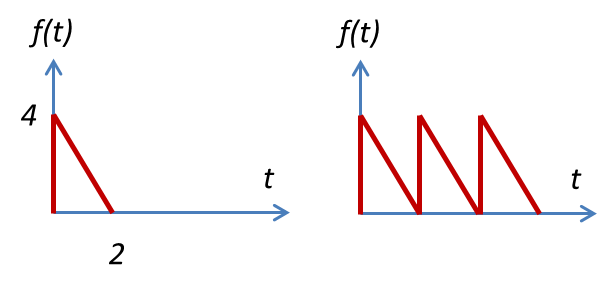
\includegraphics[width=.9\textwidth]{png/signaux}
\end{center}
\end{minipage}


\ifthenelse{\boolean{prof}}{
\begin{corrige}
On pourrait définir le premier signal ainsi : $\forall t\in [0,2], f_1(t)=4-2t$, sinon $f_1(t)=0$.

Une seconde façon serait d'utiliser la fonction de Heaviside définit par : $\forall t>0 u(t)=1$, sinon $u(t)=0$. On aurait alors  $\forall t\in ]-\infty,2], f_2(t)=\left(4-2t\right)\cdot u(t)$, sinon $f_2(t)=0$.

Enfin, dans un troisième temps on peut rechercher une fonction qui serait définie sur $\mathbb{R}$. Pour cela, définissons d'abord une fonction $g$ telle que $g(t)=\left( -4+2t\right) \cdot u(t-2)$. 

On peut donc définir $f$ ainsi : $\forall t\in \mathbb{R}, f(t)= \left(4-2t\right)\cdot u(t) + \left( -4+2t\right) \cdot u(t-2)$.


Dans le domaine de Laplace, on a donc :
$$
F(p)= \dfrac{4}{p}-\dfrac{2}{p^2} +e^{-2p}\left(- \dfrac{4}{p}+\dfrac{2}{p^2}\right)
$$


Enfin, si le signal est 2-périodique, on obtient : 
$$
F(p)= \dfrac{\dfrac{4}{p}-\dfrac{2}{p^2} +e^{-2p}\left(- \dfrac{4}{p}+\dfrac{2}{p^2}\right)}{1-e^{-2p}}
$$


\end{corrige}
}{}

\subsection*{Exercice 3 -- Système mécanique}
\setcounter{subparagraph}{0}
\begin{minipage}[c]{.6\linewidth}
Soit le système mécanique ci-contre constitué d'un ressort de raideur $k$ et d'un amortisseur de coefficient d'amortissement $f$. On peut déplacer l'extrémité du ressort $A$ d'une quantité $x$. \'A l'instant $t=0$ le système est en équilibre, le point $A$ est positionné en $x_0$ et le point $B$ est positionné en $y_0$. 

On notera $x(t)$ et $y(t)$ les variations des positions des points $A$ et $B$ autour de $x_0$ et $y_0$.


\end{minipage}\hfill
\begin{minipage}[c]{.35\linewidth}
\begin{center}
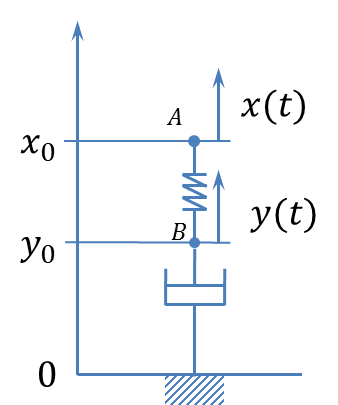
\includegraphics[width=.9\textwidth]{png/systeme_meca}
\end{center}
\end{minipage}


\subparagraph{}
\textit{Donner l'équation différentielle faisant intervenir $x(t)$ et $y(t)$. $K$ désigne la raideur du ressort, $f$ désigne le coefficient visqueux de l'amortisseur. La pièce liant ressort et amortisseur au point $B$ est considérée comme ayant une masse quasiment nulle.}
\ifthenelse{\boolean{prof}}{
\begin{corrige}
En appliquant le théorème de la résultante dynamique en projection sur l'axe $\vect{x}$ au système ressort -- amortisseur, on obtient : 
$$
k\left(x(t)-y(t)\right) - f\dfrac{dy(t)}{dt} = M \dfrac{dy^2(t)}{dt^2}
$$

Dans notre cas, la masse du système isolée est nulle. On a donc : 
$$
k\left(x(t)-y(t)\right) = f\dfrac{dy(t)}{dt}
$$

\end{corrige}
}{}




\subparagraph{}
\textit{Réécrire cette équation en passant du domaine temporel au domaine de Laplace.}
\ifthenelse{\boolean{prof}}{
\begin{corrige}
Dans le domaine de Laplace, on a donc directement :
$$
k\left(X(p)-Y(p)\right) = fpY(p)
$$
\end{corrige}
}{}

\subparagraph{}
\textit{Déterminer la fonction $H(p)=\dfrac{Y(p)}{X(p)}$. $H$ sera appelée fonction de transfert du système.}
\ifthenelse{\boolean{prof}}{
\begin{corrige}
Il vient directement : 
$$
H(p)=\dfrac{Y(p)}{X(p)} = \dfrac{K}{K+fp}
$$
\end{corrige}
}{}

\subparagraph{}
\textit{Donner la réponse du système à un échelon unitaire puis mettre $S(p)$ sous la forme $S(p)=\dfrac{1}{p}\cdot\dfrac{1}{A+\tau p}$. On précisera l'expression de $\tau$. }
\ifthenelse{\boolean{prof}}{
\begin{corrige}
L'entrée du système correspond à la position de $A$ et la sortie à la position de $B$. 

Si on sollicite le système par un échelon de position, on a donc $X(p)=\dfrac{1}{p}$: 
$$
Y(p)=H(p) \cdot X(p) = \dfrac{k}{k+fp}\cdot \dfrac{1}{p}
= \dfrac{1}{1+\dfrac{f}{k}p}\cdot \dfrac{1}{p}
$$
On pose alors $\tau = \dfrac{f}{k}$
\end{corrige}
}{}


\subparagraph{}
\textit{Mettre $Y(p)$ sous la forme $\dfrac{\alpha}{p}+\dfrac{\beta }{1+\tau p}$.}
\ifthenelse{\boolean{prof}}{
\begin{corrige}
Posons :
$$
Y_1(p)=\dfrac{1}{1+\tau p}\cdot \dfrac{1}{p} 
\quad \text{et} \quad
Y_2(p)=\dfrac{\alpha}{p}+\dfrac{\beta }{1+\tau p} 
\quad \text{avec} \quad 
Y_1(p)=Y_2(p)
$$

On multiplie $Y_1$ et $Y_2$ par $p$ et on pose $p=0$. On obtient alors $\alpha=1$.

On multiplie ensuite $Y_1$ et $Y_2$ par $1+\tau p$ et on pose $p=-\dfrac{1}{\tau}$. On obtient alors $\beta=-\tau$.

On obtient donc :
$$
Y(p)=\dfrac{1}{p}-\dfrac{\tau}{1+\tau p}
$$
\end{corrige}
}{}


\subparagraph{}
\textit{En déduire la réponse $y(t)$ à un échelon unitaire.}
\ifthenelse{\boolean{prof}}{
\begin{corrige}
On modifie $Y(p)$ pour la mettre sous une forme connue : 
$$
Y(p)=\dfrac{1}{p}-\dfrac{1}{\dfrac{1}{\tau}+p}
$$

Dans le domaine temporel, on a donc : 
$$
y(t)=u(t)\cdot\left(1-e^{-\dfrac{t}{\tau}}\right)
$$
\end{corrige}
}{}


\subparagraph{}
\textit{Tracer graphiquement l'allure générale de $y(t)$. }
\ifthenelse{\boolean{prof}}{
\begin{corrige}

\end{corrige}
}{}


\subparagraph{}
\textit{Recommencer le même travail en étudiant la réponse du système à une entrée sinusoïdale $e(t)=\sin\left( \omega\cdot t\right)\cdot u(t)$ avec $\omega = 1 rad/s$ et $T=\dfrac{f}{K}=1$. On fera donc l'hypothèse que le système est particulier, c'est-à-dire que $T=1$.}
\ifthenelse{\boolean{prof}}{
\begin{corrige}
En appliquant $x(t)=\sin (t)$, on a : 
$$
Y(p)=\dfrac{1}{1+p}\cdot\dfrac{1}{p^2+1} 
= \dfrac{1}{2}\cdot \left[ \dfrac{1}{1+p} - \dfrac{p-1}{p^2+1} \right]
= \dfrac{1}{2}\cdot \left[ \dfrac{1}{1+p} - \dfrac{p}{p^2+1} + \dfrac{1}{p^2+1} \right]
$$
On a donc dans le domaine temporel : 
$$
y(t)=\dfrac{1}{2} \left[ e^{-t} - \cos t + \sin t\right]
$$

Remarque : 
$$
\sin t - \cos t = \sin t - \cos t \cdot\dfrac \tan {\pi}{4}
 = \sin t - \cos t \dfrac{\sin {\pi}{4}}{\cos {\pi}{4}}
 = \sqrt{2}\left( \sin t \cos \dfrac{\pi}{4} - \cos t \sin \dfrac{\pi}{4} \right)
 = \sqrt{2} \sin \left( t - \dfrac{\pi}{4}\right)
$$

Au final :
$$y(t) = \dfrac{1}{2} \left[ e^{-t} + \sqrt{2} \sin \left(t-\dfrac{\pi}{4} \right)\right]$$
\end{corrige}
}{}



\subsection*{Exercice 4 -- Transformée de Laplace}
\setcounter{subparagraph}{0}
Connaissant les transformées de Laplace des fonctions $\cos (\omega t)\cdot u(t)$, donner la transformée de Laplace de $e^{-at}\cdot\cos (\omega t)\cdot u(t)$.


\subsection*{Exercice 5 -- Transformée de Laplace inverse}
\setcounter{subparagraph}{0}
Calculer les transformées de Laplace inverses des fonctions suivantes :
$$
\begin{array}{ccc}
F_1(p)= \dfrac{K_1}{\left( p+a \right) \cdot \left(p+b \right)} & 
F_2(p)= \dfrac{K_2}{p\cdot \left(1+\tau p \right)} &
F_3(p)= \dfrac{K_3 \cdot p}{\left(p+	a\right)\left(p+b\right)}  \\
F_4(p)= \dfrac{K_4 p^2}{\left( p-1 \right)^2 \cdot \left(p+1\right)} & 
F_5(p)= \dfrac{3p+1}{\left(p-1\right)\cdot \left(p^2+1\right)} 
\end{array}
$$


\subsection*{Exercice 6 -- Circuit RLC}
\setcounter{subparagraph}{0}
\begin{minipage}[c]{.7\linewidth}
On donne le schéma électrique ci-contre. On suppose que les conditions initiales sont nulles. 

\subparagraph{}
\textit{Déterminer l'équation différentielle liant $u_c(t)$ et $e(t)$.}

\subparagraph{}
\textit{$e(t)$ étant un échelon d'amplitude $E_0$, résoudre l'équation en utilisant la transformée de Laplace.}
\end{minipage} \hfill
\begin{minipage}[c]{.25\linewidth}
\begin{center}
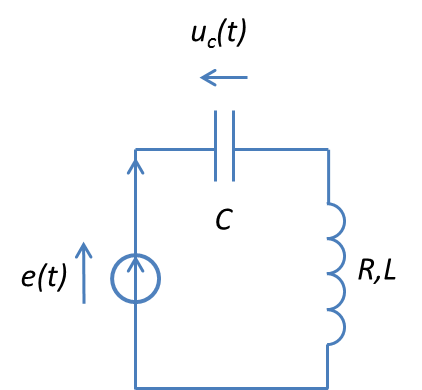
\includegraphics[width=.95\textwidth]{png/RLC.png}
\end{center}
\end{minipage}

\subsection*{Exercice 7 -- Transformées de Laplace inverse}
\setcounter{subparagraph}{0}
On donne les fonctions suivantes : 
$$
F_1(p)= \dfrac{3}{p\cdot \left(p+1\right)\cdot \left(p+2\right)} \quad
F_2(p)= \dfrac{2p +1}{p^2 + 2p + 10} 
$$

\subparagraph{}
\textit{En utilisant la transformées de Laplace inverse, donner les fonctions causales du temps.}

\subsection*{Exercice 8}
\setcounter{subparagraph}{0}
Soit la fonction de transfert suivante : 
$$ H(p) = \dfrac{p^2+1}{p^2\left(p+1\right)}$$. 
On fait subir au système représenté par cette fonction de transfert une entrée échelon unitaire. 

\subparagraph{}
\textit{Calculer $S(p)$ la réponse du système.}

\subparagraph{}
\textit{Décomposer là en éléments simples sous la forme : $\dfrac{A}{p^3}+\dfrac{B}{p^2}+\dfrac{C}{p}+\dfrac{D}{p+1}$.}

\subparagraph{}
\textit{Déterminer $s(t)$.}

\subparagraph{}
\textit{Réaliser un tracé représentatif de la fonction $s(t)$.}


\subsection*{Équation différentielle}
\setcounter{subparagraph}{0}
Il s'agit de résoudre l'équation différentielle suivante : 

$$
\dfrac{d^2y(t)}{dt^2}+3\dfrac{dy(t)}{dt}+2y(t) = e(t) \quad \text{avec} \quad y(0)=2\quad \dfrac{dy(0)}{dt}=2
$$

Par ailleurs, $e(t)=6\cdot u(t)$.

\subparagraph{}
\textit{Écrire cette équation à l'aide de la transformée de Laplace.}


\subparagraph{}
\textit{Décomposer $Y(p)$ sous la forme $\dfrac{A}{p}+\dfrac{B}{p+\alpha}+\dfrac{C}{p+\beta}$.}

\subparagraph{}
\textit{Donner une représentation graphique de $y(t)$.}




%\subparagraph{}
%\textit{}
%\ifthenelse{\boolean{prof}}{
%\begin{corrige}
%
%\end{corrige}
%}{}


\end{document}
